\documentclass[11pt]{article}
% Self-contained copy of the lecture style for the built-in editor.
\RequirePackage[margin=1in]{geometry}
\RequirePackage{fontspec,unicode-math,amsmath,amsthm,tikz-cd,booktabs,xcolor,titlesec,needspace,hyperref}
\setmainfont{texgyretermes}[Extension=.otf,UprightFont=*-regular,BoldFont=*-bold,ItalicFont=*-italic,BoldItalicFont=*-bolditalic]
\setmathfont{texgyretermes-math.otf}
\definecolor{teal}{HTML}{176568}
\definecolor{burgundy}{HTML}{782F40}
\hypersetup{colorlinks=true,linkcolor=teal,urlcolor=teal,pdfstartview={XYZ null null 1.5}}
\setlength{\parindent}{0pt}\setlength{\parskip}{4pt plus .5pt minus .5pt}
\newcommand{\facehead}[1]{\par\Needspace{4\baselineskip}\subsection{#1}}
\newcommand{\facecase}[1]{\par\Needspace{4\baselineskip}\smallskip\textbf{#1.}\par}
\newcommand{\Z}{\mathbb Z}

\titleformat{\section}{\large\bfseries\color{teal}}{\thesection}{1em}{}
\titleformat{\subsection}{\normalsize\bfseries\color{burgundy}}{\thesubsection}{.65em}{}
\titlespacing*{\section}{0pt}{2.2ex plus .5ex minus .2ex}{1ex plus .2ex}
\titlespacing*{\subsection}{0pt}{1.6ex plus .4ex minus .2ex}{.7ex plus .2ex}
\setcounter{tocdepth}{2}
\hypersetup{pdftitle={Lecture 6: Homotopy Invariance and First Computations},pdfauthor={Math 615},pdfsubject={Revision 20}}

\raggedbottom
\begin{document}
\begin{center}
{\Large\bfseries Lecture 6}\\[4pt]
{\LARGE\bfseries Homotopy Invariance and First Computations}\\[6pt]
Math 615: Algebraic Topology I\\Fall 2026
\end{center}
We first study homotopy invariant functors and the homotopy category of spaces. Singular homology is the main example: homotopies of spaces induce chain homotopies of singular chains. We prove this by triangulating a prism, then compute the homology of points, discrete spaces, and contractible spaces. Relative chains provide the first computation in positive degree: an interval has no absolute first homology, but it has a relative first homology class when its endpoints are placed in the subspace.

Throughout, coefficients are integers, chain complexes are homologically graded, and groups in negative degrees are zero. We write $I=[0,1]$ for the interval. The singular chain functor is the one constructed in Lecture 5 from the singular simplicial set and the degreewise free abelian group functor.
{\setlength{\parskip}{0pt}\small\tableofcontents}
\section{General Homotopy Invariance}\label{sec:definitions}
Homotopy invariant functors identify homotopic maps and send homotopy equivalences to isomorphisms. We first establish these general facts, then recall the corresponding algebraic statement for chain complexes.

\Needspace{10\baselineskip}
\facehead{Homotopies and Homotopy Equivalences}
\textbf{Definition 1.1.} A homotopy from $f:X\to Y$ to $g:X\to Y$ is a continuous map $h:X\times I\to Y$ making both triangles commute:
\[
\begin{tikzcd}
X \arrow[r,"j_0"] \arrow[dr,"f"'] & X\times I \arrow[d,"h"] & X\arrow[l,"j_1"']\arrow[dl,"g"]\\
&Y&
\end{tikzcd}
\]
Here $j_0(x)=(x,0)$ and $j_1(x)=(x,1)$. A homotopy equivalence is a map $f:X\to Y$ admitting $g:Y\to X$ such that $gf$ and $fg$ are homotopic to the respective identity maps. A nonempty space is contractible if its identity map is homotopic to a constant map.

\facehead{The Homotopy Category and Homotopy Invariant Functors}
Write $\mathrm{Top}$ for the category of topological spaces and continuous maps, and write $f\simeq g$ when the maps $f,g:X\to Y$ are homotopic. Constant homotopies, reversal of the interval, and concatenation show that $\simeq$ is an equivalence relation.

\hypertarget{def:htop}{}\textbf{Definition 1.2.} The \emph{homotopy category of spaces} $\mathrm{hTop}$ has topological spaces as objects and
\[
\operatorname{Mor}_{\mathrm{hTop}}(X,Y)
=\{\text{continuous maps }X\to Y\}/\simeq.
\]
For a continuous map $f:X\to Y$, write $[f]$ for its homotopy class. The identity of $X$ is $[\mathrm{id}_X]$, and composition is
\[
[g]\circ[f]=[g\circ f]
\quad(f:X\to Y,\ g:Y\to Z).
\]
Composition is well defined: if $f_0\simeq f_1:X\to Y$ and $g_0\simeq g_1:Y\to Z$, then
\[
g_0f_0\simeq g_0f_1\simeq g_1f_1.
\]
Associativity and the identity laws follow from those for continuous maps. The quotient functor $q:\mathrm{Top}\to\mathrm{hTop}$ is the identity on objects and satisfies $q(f)=[f]$.

\hypertarget{def:homotopy-invariant}{}\textbf{Definition 1.3.} Let $C$ be a category. A functor $F:\mathrm{Top}\to C$ is \emph{homotopy invariant} if, for all spaces $X,Y$ and continuous maps $f,g:X\to Y$,
\[
f\simeq g\quad\Longrightarrow\quad F(f)=F(g):F(X)\longrightarrow F(Y).
\]
Equivalently, $F$ factors uniquely through $q$:
\[
\begin{tikzcd}
\mathrm{Top}\arrow[r,"q"]\arrow[dr,"F"']&\mathrm{hTop}\arrow[d,"\overline F"]\\
&C.
\end{tikzcd}
\]
Indeed, homotopy invariance makes $\overline F(X)=F(X)$ and $\overline F([f])=F(f)$ well defined. These formulas define a functor and are forced by $F=\overline Fq$. Conversely, such a factorization gives $F(f)=F(g)$ whenever $[f]=[g]$.

\hypertarget{prop:homotopy-invariant}{}\textbf{\hyperlink{proof:homotopy-invariant}{Proposition 1.4.}} Every homotopy invariant functor $F:\mathrm{Top}\to C$ sends homotopy equivalences to isomorphisms.

\hypertarget{proof:homotopy-invariant}{}\textbf{\hyperlink{prop:homotopy-invariant}{Proof.}} Let $f:X\to Y$ be a homotopy equivalence with homotopy inverse $g:Y\to X$. Since $gf\simeq\mathrm{id}_X$ and $fg\simeq\mathrm{id}_Y$, functoriality and homotopy invariance give
\[
\begin{aligned}
F(g)\circ F(f)&=F(gf)=F(\mathrm{id}_X)=\mathrm{id}_{F(X)},\\
F(f)\circ F(g)&=F(fg)=F(\mathrm{id}_Y)=\mathrm{id}_{F(Y)}.
\end{aligned}
\]
Thus $F(f)$ is an isomorphism with inverse $F(g)$.\hfill$\mdlgwhtsquare$

In particular, $[f]$ is an isomorphism in $\mathrm{hTop}$ if and only if $f$ is a homotopy equivalence: a class $[g]$ is inverse to $[f]$ exactly when $gf\simeq\mathrm{id}_X$ and $fg\simeq\mathrm{id}_Y$.

\facehead{Chain Homotopies}

Let $(A_\bullet,d_A)$ and $(B_\bullet,d_B)$ be chain complexes. For chain maps $u,v:A_\bullet\to B_\bullet$, a chain homotopy from $u$ to $v$ is a family $K_n:A_n\to B_{n+1}$ satisfying
\[v-u=d_BK+Kd_A.\]
On a cycle $z$, this says $v(z)-u(z)=d_BK(z)$, so $u_*=v_*$. A chain homotopy equivalence is a chain map $u:A_\bullet\to B_\bullet$ with a chain map $r:B_\bullet\to A_\bullet$ such that $ru$ and $ur$ are chain homotopic to the respective identities. Passing to homology gives $r_*u_*=\mathrm{id}$ and $u_*r_*=\mathrm{id}$, so $u_*$ is an isomorphism with inverse $r_*$. This is the algebraic principle we apply to a topological homotopy.

\section{Singular Homology}\label{sec:singular-homology}
We show that singular homology is homotopy invariant by constructing a chain homotopy from a homotopy of spaces. The construction triangulates the prism over each standard simplex.

\facehead{Singular Chains}
The standard topological $n$-simplex is
\[
\lvert\Delta^n\rvert
=\left\{(t_0,\ldots,t_n)\in\mathbb R^{n+1}:t_i\ge0,\ \sum_{i=0}^nt_i=1\right\},
\]
Its vertices $e_0,\ldots,e_n$ are the standard basis vectors of $\mathbb R^{n+1}$.
The numbers $t_i$ are the barycentric coordinates of $x=\sum_i t_ie_i$.
A singular $n$-simplex of $X$ is a continuous map $\sigma:\lvert\Delta^n\rvert\to X$.

The group $C_n(X)$ is free abelian on these maps. We also write $\sigma$ for the corresponding generator of $C_n(X)$.
For $n\ge1$ and $0\le k\le n$, the affine face inclusion is
\[
\begin{aligned}
d^k:\lvert\Delta^{n-1}\rvert&\longrightarrow\lvert\Delta^n\rvert,\\
(t_0,\ldots,t_{n-1})&\longmapsto(t_0,\ldots,t_{k-1},0,t_k,\ldots,t_{n-1}).
\end{aligned}
\]
The singular differential is
\[
\partial\sigma=\sum_{k=0}^n(-1)^k\sigma d^k\quad(n\ge1),
\qquad \partial:C_0(X)\longrightarrow0.
\]
The face identities give $\partial^2=0$, as proved in Lecture 5. A cycle is a chain with zero boundary, and $H_n(X)$ is the group of cycles modulo boundaries. Postcomposition by $f:X\to Y$ induces the chain map $f_\#$ and the homology map $f_*$.

The following prism construction gives the chain homotopy explicitly; see also [1, Theorem 2.10].

\label{sec:result}\hypertarget{thm12}{}\textbf{\hyperlink{proof12}{Theorem 2.1.}} Let $f,g:X\to Y$ be continuous maps and let $h:X\times I\to Y$ be a homotopy from $f$ to $g$. Then the induced singular chain maps $f_\#,g_\#:C_\bullet(X)\to C_\bullet(Y)$ are chain homotopic. In particular, $f_*=g_*$ on singular homology, and every homotopy equivalence induces isomorphisms in all degrees.

\label{sec:details}\hypertarget{proof12}{}\textbf{\hyperlink{thm12}{Proof.}} We triangulate each prism $\lvert\Delta^n\rvert\times I$ so that its boundary consists of the top, minus the bottom, minus the prisms on the boundary of $\lvert\Delta^n\rvert$. Composing with $h(\sigma\times\mathrm{id}_I)$ gives the required chain homotopy.

\facehead{The Affine Prism Simplices}
For $0\le j\le n$, let
\[
\tau_j^n:\lvert\Delta^{n+1}\rvert\longrightarrow\lvert\Delta^n\rvert\times I
\]
be the unique affine map with ordered vertices
\[
\bigl[(e_0,0),\ldots,(e_j,0),(e_j,1),\ldots,(e_n,1)\bigr].
\]
Here $e_k$ denotes the standard basis vector in the Euclidean space containing the indicated simplex. On the standard vertices of the source,
\[
\tau_j^n(e_k)=
\begin{cases}
(e_k,0),&0\le k\le j,\\
(e_{k-1},1),&j+1\le k\le n+1.
\end{cases}
\]
Thus, for barycentric coordinates $(u_0,\ldots,u_{n+1})$ in the source,
\[
\tau_j^n(u_0,\ldots,u_{n+1})=
\left(\sum_{k=0}^{j}u_ke_k+\sum_{k=j+1}^{n+1}u_ke_{k-1},\;
\sum_{k=j+1}^{n+1}u_k\right).
\]
We retain $s_k=(e_k,0)$ for the bottom vertices; top vertices are written $(e_k,1)$.

For $x=\sum_{i=0}^nt_ie_i$ and $t\in I$, the point $(x,t)$ lies in the image of $\tau_j^n$ exactly when
\[
\sum_{i>j}t_i\le t\le\sum_{i\ge j}t_i.
\]
Indeed, its unique preimage then has coordinates
\[
u_k=
\begin{cases}
t_k,&k<j,\\
\displaystyle\sum_{i\ge j}t_i-t,&k=j,\\
\displaystyle t-\sum_{i>j}t_i,&k=j+1,\\
t_{k-1},&k>j+1.
\end{cases}
\]
These coordinates are nonnegative and sum to one. The intervals above cover $[0,1]$ because the successive partial sums run from $0$ to $1$. For $j<\ell$, the two images meet in the face with ordered vertices
\[
\bigl[(e_0,0),\ldots,(e_j,0),(e_\ell,1),\ldots,(e_n,1)\bigr].
\]
In fact, membership in both images forces $t=\sum_{i>j}t_i=\sum_{i\ge\ell}t_i$ and $t_{j+1}=\cdots=t_{\ell-1}=0$. This proves that the images form a triangulation.

For $n=1$, its two triangles and their common diagonal are:
\[
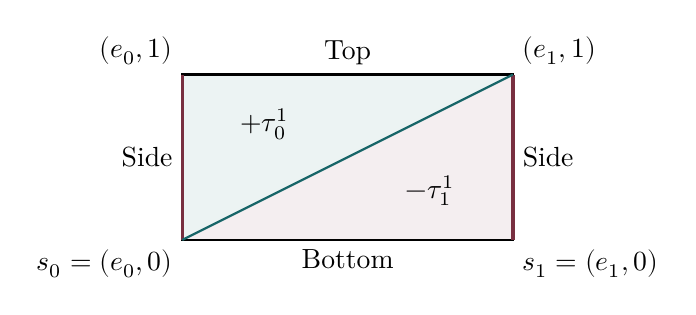
\begin{tikzpicture}[scale=1.05,>=stealth]
\fill[teal!8] (0,0)--(0,2)--(4,2)--cycle;
\fill[burgundy!8] (0,0)--(4,0)--(4,2)--cycle;
\draw[thick] (0,0)--(4,0)--(4,2)--(0,2)--cycle;
\draw[very thick,burgundy] (0,0)--(0,2) (4,0)--(4,2);
\draw[thick,teal] (0,0)--(4,2);
\node[below left] at (0,0) {$s_0=(e_0,0)$};
\node[below right] at (4,0) {$s_1=(e_1,0)$};
\node[above left] at (0,2) {$(e_0,1)$};
\node[above right] at (4,2) {$(e_1,1)$};
\node at (1,1.4) {$+\tau_0^1$};
\node at (3,.6) {$-\tau_1^1$};
\node[above] at (2,2) {Top};
\node[below] at (2,0) {Bottom};
\node[left] at (0,1) {Side};
\node[right] at (4,1) {Side};
\end{tikzpicture}
\]
The diagonal $[(e_0,0),(e_1,1)]$ joins vertices over both endpoints of the base; its open segment lies inside the square. Each vertical side lies over just one endpoint of the base.

\facehead{The Prism Operator}
For a singular simplex $\sigma:\lvert\Delta^n\rvert\to X$, define $\sigma_j$ by the composite
\begin{equation*}\label{diag:prism-composite}
\begin{tikzcd}[column sep=small]
\lvert\Delta^{n+1}\rvert\arrow[r,"\tau_j^n"]&
\lvert\Delta^n\rvert\times I\arrow[r,"\sigma\times\mathrm{id}_I"]&
X\times I\arrow[r,"h"]&Y.
\end{tikzcd}
\end{equation*}
By freeness, define $P_n:C_n(X)\to C_{n+1}(Y)$ on generators by
\[
\sigma\longmapsto\sum_{j=0}^n(-1)^j\sigma_j.
\]
Set $P_{-1}=0$.

\facehead{Faces of the Prism}
In $\partial P_n$, deleting the vertex in position $r$ of $\tau_j^n$ has coefficient $(-1)^{j+r}$. We classify every such face.

These are the $n$-dimensional faces obtained by deleting one vertex. In coordinates $(x,t)$, with $x=\sum_i t_i e_i$, the interior of the prism in its affine span is described by
\[
t_i>0\quad\text{for every }i,\qquad 0<t<1.
\]
Its vertical boundary consists of the points where at least one base coordinate $t_k$ is zero.

\facecase{Top and Bottom Faces}
The two end faces are given by the following table. Here $\iota_\epsilon(x)=(x,\epsilon)$ for $\epsilon\in\{0,1\}$.
\[
\begin{array}{c c c c}
\text{Face}&\text{Deleted Vertex}&\text{Affine Map}&\text{Coefficient}\\\hline
\text{Top}&(e_0,0)\text{ in }\tau_0^n&\tau_0^n d^0=\iota_1&+1\\
\text{Bottom}&(e_n,1)\text{ in }\tau_n^n&\tau_n^n d^{n+1}=\iota_0&(-1)^{2n+1}=-1
\end{array}
\]
After composition with $h(\sigma\times\mathrm{id}_I)$, their contribution is
\[
g\sigma-f\sigma
=(g_\#-f_\#)\sigma.
\]

\facecase{Interior Faces}
For $0\le j<n$, delete $(e_j,1)$ from $\tau_j^n$, or delete $(e_{j+1},0)=s_{j+1}$ from $\tau_{j+1}^n$. In both cases the remaining ordered vertices are
\[
\bigl[(e_0,0),\ldots,(e_j,0),(e_{j+1},1),\ldots,(e_n,1)\bigr].
\]
There is still one vertex over every $e_k$, and both bottom and top vertices remain. A point with positive barycentric coordinates on this face therefore satisfies
\[
t_k>0\quad(0\le k\le n),\qquad
t=\sum_{k=j+1}^n t_k\in(0,1).
\]
Thus the relative interior of this face lies inside the prism: it separates two pieces of the triangulation there. Its own boundary can still meet the boundary of the prism, as the endpoints of the diagonal do in the square.

Both deleted vertices occupy position $j+1$. Equality on standard vertices gives the commutative square
\begin{equation*}\label{diag:interior}
\begin{tikzcd}
\lvert\Delta^n\rvert\arrow[r,"d^{j+1}"]\arrow[d,"d^{j+1}"']&
\lvert\Delta^{n+1}\rvert\arrow[d,"\tau_j^n"]\\
\lvert\Delta^{n+1}\rvert\arrow[r,"\tau_{j+1}^n"']&
\lvert\Delta^n\rvert\times I.
\end{tikzcd}
\end{equation*}
The coefficients of this common ordered face are
\[
\underbrace{(-1)^j(-1)^{j+1}}_{-1}
\quad\text{and}\quad
\underbrace{(-1)^{j+1}(-1)^{j+1}}_{+1}.
\]
Thus the two signed prism simplices induce opposite orientations on their common face. Their boundaries cancel. After composition with $h(\sigma\times\mathrm{id}_I)$, they are still the same parametrized singular simplex with opposite coefficients.

\facecase{Side Faces}
The $k$th face of the base is $t_k=0$. Every point of a face is a convex combination of its vertices. If none of those vertices lies over $e_k$, its $k$th base coordinate is therefore always zero. The whole face lies in the vertical boundary over the $k$th base face.

In $\tau_j^n$, the base vertex $e_j$ occurs at both heights; every other $e_k$ occurs at just one height. Deleting the only vertex over such an $e_k$ gives a side face. Deleting one of the two vertices over $e_j$ still leaves every base vertex represented, giving an interior face except in the top and bottom cases already listed. For $n\ge1$, the side cases are:
\[
\begin{array}{c c c c c}
\text{Deleted Vertex}&r&\ell&\text{In }\partial P_n&\text{In }P_{n-1}\partial\\\hline
(e_k,0)=s_k,\ k<j&k&j-1&(-1)^{j+k}&(-1)^{j+k-1}\\
(e_k,1),\ k>j&k+1&j&(-1)^{j+k+1}&(-1)^{j+k}
\end{array}
\]
Here $r$ is the deleted position and $\ell$ is the transition index in the prism on the base face. Omitting $e_k$ renumbers the later base vertices; in both rows equality on standard vertices gives
\begin{equation*}\label{diag:sides}
\begin{tikzcd}
\lvert\Delta^n\rvert\arrow[r,"d^r"]\arrow[d,"\tau_\ell^{n-1}"']&
\lvert\Delta^{n+1}\rvert\arrow[d,"\tau_j^n"]\\
\lvert\Delta^{n-1}\rvert\times I\arrow[r,"d^k\times\mathrm{id}_I"']&
\lvert\Delta^n\rvert\times I.
\end{tikzcd}
\end{equation*}
Every term of $P_{n-1}\partial\sigma$ occurs once: for its indices $(k,\ell)$, use $j=\ell+1$ if $k\le\ell$, and $j=\ell$ if $k>\ell$. The two sign columns are opposite. Hence the total side contribution is $-P_{n-1}\partial\sigma$.

\facehead{The Chain-Homotopy Identity}
Deleting either vertex over $e_j$ gives an interior face, except for the top at $j=0$ and the bottom at $j=n$. Every other deletion gives a side face. The classification is exhaustive, so
\[
\begin{aligned}
\partial P_n\sigma
&=\underbrace{(g_\#-f_\#)\sigma}_{\text{Top and Bottom}}
\;\underbrace{-P_{n-1}\partial\sigma}_{\text{Sides}}
\;+\underbrace{0}_{\text{Interior}}.
\end{aligned}
\]
For $n=0$, $\tau_0^0$ is just the interval with its two endpoints, so the same formula holds. By freeness,
\begin{equation}\label{eq:chain-homotopy}
\partial P_n+P_{n-1}\partial=g_\#-f_\#,\qquad P_{-1}=0.\tag{1}
\end{equation}
For a cycle $z$, this gives $g_\#z-f_\#z=\partial P_nz$, hence $f_*[z]=g_*[z]$. Thus $H_n:\mathrm{Top}\to\mathrm{Ab}$ is homotopy invariant, where $\mathrm{Ab}$ denotes the category of abelian groups. By \hyperlink{prop:homotopy-invariant}{Proposition 1.4}, it sends homotopy equivalences to isomorphisms.\hfill$\mdlgwhtsquare$


The universal property of $\hyperlink{def:htop}{\mathrm{hTop}}$ now gives the unique factorization
\[
\begin{tikzcd}
\mathrm{Top}\arrow[r,"q"]\arrow[dr,"H_n"']&\mathrm{hTop}\arrow[d,"\overline H_n"]\\
&\mathrm{Ab}.
\end{tikzcd}
\]

\Needspace{8\baselineskip}
\section{First Absolute Computations}
We first show that homology preserves disjoint unions. We then compute a point and path components directly from the differential. Homotopy invariance computes every contractible space.

\facehead{Disjoint Unions}
\hypertarget{disjoint-theorem}{}\textbf{\hyperlink{disjoint-proof}{Theorem (Homology of Disjoint Unions).}} For any set-indexed family of topological spaces $(X_i)_{i\in J}$, the inclusions into the disjoint union induce a natural isomorphism of graded abelian groups
\[
\bigoplus_{i\in J}H_*(X_i)\ \xrightarrow{\ \cong\ }\ H_*\!\left(\coprod_{i\in J}X_i\right).
\]
The direct sum on the left is taken in graded abelian groups: in degree $n$ it is $\bigoplus_{i\in J}H_n(X_i)$. The coproduct on the right is the topological disjoint union. The statement includes the empty family.

\hypertarget{disjoint-proof}{}\textbf{\hyperlink{disjoint-theorem}{Proof.}} A singular simplex $\sigma:\lvert\Delta^n\rvert\to\coprod_iX_i$ has connected, nonempty domain. Each summand is open and closed in the disjoint union, so the image of $\sigma$ lies in exactly one $X_i$. Thus the set of singular $n$-simplices of the union is the disjoint union of the sets of singular $n$-simplices of the summands. Taking free abelian groups gives
\[
\bigoplus_iC_n(X_i)\ \xrightarrow{\ \cong\ }\ C_n\!\left(\coprod_iX_i\right).
\]
Every face of a simplex remains in the same summand. These isomorphisms therefore commute with the differentials and identify the singular chain complex of the union with $\bigoplus_iC_\bullet(X_i)$.

The differential acts separately on each summand. Since every chain in a direct sum has finite support, its boundary is zero exactly when each component has zero boundary, and a finite family of boundaries admits a finite family of preimages. Consequently
\[
Z_n\!\left(\bigoplus_iC_\bullet(X_i)\right)=\bigoplus_i Z_n(X_i),
\qquad
B_n\!\left(\bigoplus_iC_\bullet(X_i)\right)=\bigoplus_i B_n(X_i).
\]
Taking the quotient of cycles by boundaries proves the assertion in every degree. The maps are induced by the summand inclusions, so the isomorphism is natural. For the empty family both chain complexes and all homology groups are zero.\hfill$\mdlgwhtsquare$

\facehead{Path Components}
Write $\pi_0^{\mathrm{path}}(X)$ for the set of path components: two points are equivalent if a continuous path joins them. For a set $E$, write $\mathbb Z[E]$ for the free abelian group on $E$.

\hypertarget{prop21}{}\textbf{\hyperlink{proof21}{Proposition 3.1.}} For every topological space $X$, the assignment of a point to its path component induces a natural isomorphism
\[H_0(X)\cong\mathbb Z[\pi_0^{\mathrm{path}}(X)].\]
\hypertarget{proof21}{}\textbf{\hyperlink{prop21}{Proof.}} We identify the universal property of $H_0(X)$. Let $M$ be an abelian group. By freeness, a homomorphism $\alpha:C_0(X)\to M$ is an assignment of an element of $M$ to each point of $X$. Since the boundary of a path is its endpoint minus its starting point, $\alpha\partial=0$ means that this assignment is constant on path components. The cokernel property gives a unique factorization
\[
\begin{tikzcd}
C_1(X)\arrow[r,"\partial"]&C_0(X)\arrow[r,"q"]\arrow[dr,"\alpha"']&H_0(X)\arrow[d,"\overline\alpha"]\\
&&M.
\end{tikzcd}
\]

Thus maps from $H_0(X)$ to $M$ are naturally assignments of an element of $M$ to each path component. This is the defining universal property of the free abelian group on the set of path components, proving the natural isomorphism.\hfill$\mdlgwhtsquare$

\facehead{Points and Discrete Spaces}
\hypertarget{prop22}{}\textbf{\hyperlink{proof22}{Proposition 3.2.}} For a one-point space $*$, one has $H_0(*)=\mathbb Z$ and $H_n(*)=0$ for $n>0$.

\hypertarget{proof22}{}\textbf{\hyperlink{prop22}{Proof.}} There is one singular simplex in each degree, so $C_n(*)=\mathbb Z$. Every face map is the identity. The alternating sum is zero in odd degrees and the identity in positive even degrees. The complex is therefore
\[\cdots\longrightarrow\mathbb Z\xrightarrow{0}\mathbb Z\xrightarrow{\mathrm{id}}\mathbb Z\xrightarrow{0}\mathbb Z\longrightarrow0,\]
with the last copy of $\mathbb Z$ in degree zero. The stated homology follows by taking kernels modulo images.\hfill$\mdlgwhtsquare$

Every singular simplex lies in one path component because its domain is path connected. Hence the chain complex, and therefore its homology, splits as a direct sum over path components. This chain-level observation applies even when the path components are not open. In particular, a discrete space $E$ has $H_0(E)=\mathbb Z[E]$ and zero homology in positive degrees. The empty space has zero chain groups and zero homology in every degree.

\facehead{Contractible Spaces and Deformation Retractions}
\hypertarget{prop23}{}\textbf{\hyperlink{proof23}{Proposition 3.3.}} For every nonempty contractible space $X$, one has $H_0(X)\cong\mathbb Z$ and $H_n(X)=0$ for $n>0$.

\hypertarget{proof23}{}\textbf{\hyperlink{prop23}{Proof.}} Choose a point $x_0$ to which the identity contracts. Write $s:*\to X$ for inclusion at $x_0$ and $p:X\to *$ for the unique map. Then $ps=\mathrm{id}_*$ and $sp\simeq\mathrm{id}_X$. By Theorem 2.1, the triangle
\[
\begin{tikzcd}
H_n(X)\arrow[r,"p_*"]\arrow[dr,equal]&H_n(*)\arrow[d,"s_*"]\\
&H_n(X)
\end{tikzcd}
\]

commutes, and $p_*s_*=\mathrm{id}$ as well. Hence $p_*$ and $s_*$ are inverse isomorphisms. Proposition 3.2 computes their target.\hfill$\mdlgwhtsquare$

A nonempty convex subset $V\subseteq\mathbb R^m$ contracts to any chosen $a\in V$ by straight-line interpolation, $h(x,t)=(1-t)x+ta$. This computes the homology of $\mathbb R^m$, open and closed balls, intervals, and topological simplices. The same contraction works for a set star-shaped about $a$, meaning that it contains the segment from $a$ to each of its points.

A deformation retraction onto a subspace $X'\subseteq X$ is a retraction $r:X\to X'$, with inclusion $i:X'\hookrightarrow X$, together with a homotopy from $\mathrm{id}_X$ to $ir$ that fixes $X'$ pointwise. The identities $ri=\mathrm{id}_{X'}$ and $ir\simeq\mathrm{id}_X$ show that $i$ and $r$ induce inverse homology isomorphisms.

For example, $\mathbb R\setminus\{0\}$ deformation retracts onto $\{-1,1\}$: send each point to its sign and interpolate linearly. The interpolation stays within its half-line and fixes $-1,1$. Thus its degree-zero homology is $\mathbb Z^2$ and its positive-degree homology vanishes. More generally, deleting $r$ distinct points from $\mathbb R$ leaves $r+1$ contractible path components, giving $\mathbb Z^{r+1}$ in degree zero and zero in positive degrees.

\section{Relative Chains and the Interval}
A path between two distinct points is not an absolute cycle: its boundary is the difference of its endpoints. Passing to relative chains makes such a path a cycle. The quotient construction and the long exact sequence were introduced algebraically in Lecture 2; we now apply them to spaces.

\facehead{Pairs and Relative Chains}
\textbf{Definition 4.1.} A pair of spaces is a subspace inclusion $i:X'\hookrightarrow X$, also denoted $(X,X')$. The relative singular chain complex $C_\bullet(X,X')$ is the cokernel of $C_\bullet(X')\to C_\bullet(X)$ in chain complexes. Its homology is denoted $H_n(X,X')$. A map of pairs is a commutative square
\[
\begin{tikzcd}X'\arrow[r,"i"]\arrow[d,"f'"']&X\arrow[d,"f"]\\Y'\arrow[r,"j"']&Y,\end{tikzcd}
\]
where $f'$ is the restriction of $f$ to the subspace, viewed as a map to $Y'$.

A singular simplex of $X$ whose image lies in $X'$ is a singular simplex of $X'$ with its subspace topology. Thus inclusion identifies $C_\bullet(X')$ with a subcomplex, and the cokernel is the degreewise quotient $C_\bullet(X)/C_\bullet(X')$.

The universal property is useful: every chain map $u:C_\bullet(X)\to B_\bullet$ that vanishes on $C_\bullet(X')$ factors uniquely through the quotient. Equivalently, the left square is a pushout in chain complexes:
\[
\begin{tikzcd}
C_\bullet(X')\arrow[r]\arrow[d]&C_\bullet(X)\arrow[r,"u"]\arrow[d,"q"]&B_\bullet\arrow[d,equal]\\
0\arrow[r]&C_\bullet(X,X')\arrow[r,"\overline u"']&B_\bullet.
\end{tikzcd}
\]
For a map of pairs, apply this property to $C_\bullet(X)\to C_\bullet(Y)\to C_\bullet(Y,Y')$. The induced relative map is the unique one making the right square commute:
\[
\begin{tikzcd}
C_\bullet(X')\arrow[r]\arrow[d,"(f|_{X'})_\#"']&C_\bullet(X)\arrow[r,"q_X"]\arrow[d,"f_\#"]&C_\bullet(X,X')\arrow[d,"f_\#"]\\
C_\bullet(Y')\arrow[r]&C_\bullet(Y)\arrow[r,"q_Y"']&C_\bullet(Y,Y').
\end{tikzcd}
\]
Uniqueness proves compatibility with identities and composition, hence functoriality of relative chains and relative homology.

A relative cycle is represented by a chain in $X$ whose boundary lies in $X'$. Two such representatives give the same class if their difference is a boundary in $X$ plus a chain in $X'$. This is the quotient description of cycles and boundaries in the cokernel complex.

\facehead{The Long Exact Sequence}
\hypertarget{thm32}{}\textbf{\hyperlink{proof32}{Theorem 4.2.}} For every pair of spaces $(X,X')$, there is a natural long exact sequence
\[
\cdots\longrightarrow H_n(X')\xrightarrow{i_*}H_n(X)\xrightarrow{q_*}H_n(X,X')\xrightarrow{\delta}H_{n-1}(X')\longrightarrow\cdots,\tag{2}
\]
ending in $H_0(X')\to H_0(X)\to H_0(X,X')\to0$. If $c$ represents a relative cycle, then $\delta[c]=[\partial c]$.

\hypertarget{proof32}{}\textbf{\hyperlink{thm32}{Proof.}} Apply the long exact sequence of Lecture 2, Section 1, to the short exact sequence defining relative chains. The connecting map is obtained by lifting a relative cycle, taking its boundary, and factoring through the subcomplex:
\[
\begin{tikzcd}[column sep=small]
0\arrow[r]&C_n(X')\arrow[r]\arrow[d,"\partial"']&C_n(X)\arrow[r,"q"]\arrow[d,"\partial"]&C_n(X,X')\arrow[r]\arrow[d,"\partial"]&0\\
0\arrow[r]&C_{n-1}(X')\arrow[r]&C_{n-1}(X)\arrow[r,"q"']&C_{n-1}(X,X')\arrow[r]&0.
\end{tikzcd}
\]
A lift $c$ has boundary in $C_{n-1}(X')$ because the right square commutes and its quotient is zero. This boundary is a cycle since $\partial^2=0$. Changing the lift by a chain in $X'$ changes its boundary by a boundary in $X'$; changing the relative cycle by a boundary has no effect on the connecting class. The algebraic theorem gives exactness and naturality, with $\delta[c]=[\partial c]$.\hfill$\mdlgwhtsquare$

The three exactness statements have a direct geometric interpretation. An absolute cycle becomes zero relatively precisely when it is homologous in $X$ to a cycle in $X'$. A relative cycle has zero connecting class precisely when its boundary can be filled in $X'$, making it an absolute cycle after subtraction of that filling. A cycle in $X'$ becomes zero in $X$ precisely when it is the boundary of a relative cycle.

\facecase{The Interval and Its Endpoints}
\hypertarget{prop33}{}\textbf{\hyperlink{proof33}{Proposition 4.3.}} For the interval $I=[0,1]$ with boundary $\partial I=\{0,1\}$, the group $H_1(I,\partial I)$ is infinite cyclic and all other relative homology groups vanish. The singular edge $e:\lvert\Delta^1\rvert\to I$ given by $e(t_0,t_1)=t_1$ represents a generator.

\hypertarget{proof33}{}\textbf{\hyperlink{prop33}{Proof.}} The interval is contractible and its boundary is discrete. Section 3 identifies the map in degree zero by the commutative square
\[
\begin{tikzcd}
H_0(\partial I)\arrow[r,"i_*"]\arrow[d,"\cong"']&H_0(I)\arrow[d,"\cong"]\\
\mathbb Z\oplus\mathbb Z\arrow[r,"\mathrm{sum}"']&\mathbb Z.
\end{tikzcd}
\]
The long exact sequence identifies $H_1(I,\partial I)$ with the kernel of this map and $H_0(I,\partial I)$ with its cokernel. The map sends both endpoints to the unique path component of $I$. It is surjective and has kernel generated by $(-1,1)$. Thus $H_0(I,\partial I)=0$ and $\delta$ identifies $H_1(I,\partial I)$ with this infinite cyclic kernel. All higher relative groups vanish because their adjacent terms in (2) vanish.

The coefficients of $\partial e$ at $0,1$ are $(-1,1)$, so $\delta[e]=(-1,1)$. Hence $[e]$ generates the relative first homology.\hfill$\mdlgwhtsquare$

Reflection $r(t)=1-t$ interchanges the endpoints. The naturality square
\[
\begin{tikzcd}
H_1(I,\partial I)\arrow[r,"\delta"]\arrow[d,"r_*"']&H_0(\partial I)\arrow[d,"r_*"]\\
H_1(I,\partial I)\arrow[r,"\delta"']&H_0(\partial I)
\end{tikzcd}
\]
shows that it negates the relative generator: on the right, it sends endpoint minus starting point to its negative, and $\delta$ is injective. This is the homological meaning of reversing the orientation of the interval.

\facehead{Relative Homotopy Invariance}
\hypertarget{prop34}{}\textbf{\hyperlink{proof34}{Proposition 4.4.}} Let $f,g:(X,X')\to(Y,Y')$ be maps of pairs. If a homotopy $h:X\times I\to Y$ from $f$ to $g$ satisfies $h(X'\times I)\subseteq Y'$, then $f$ and $g$ induce the same maps on relative homology.

\hypertarget{proof34}{}\textbf{\hyperlink{prop34}{Proof.}} For a simplex with image in $X'$, every simplex in its prism has image in $Y'$. The prism operator of Theorem 2.1 therefore sends $C_n(X')$ to $C_{n+1}(Y')$ and descends to relative chains. Equation (1) descends as well, giving a chain homotopy between the relative chain maps. Thus the induced maps on relative homology agree.\hfill$\mdlgwhtsquare$

The condition on the homotopy matters. The contraction $h(x,t)=(1-t)x$ of the interval to $0$ moves the endpoint $1$ through the interior. It is not a homotopy of the pair $(I,\partial I)$: a homotopy to the constant map as maps of this pair would contradict Proposition 4.3 and Proposition 4.4.

More generally, let $X$ be a nonempty contractible space and let $X'\subseteq X$ be a nonempty finite discrete subspace with $r$ points. The same long exact sequence identifies $H_1(X,X')$ with the kernel of summation $\mathbb Z^r\to\mathbb Z$, a free abelian group of rank $r-1$; all other relative groups vanish. After choosing one point of $X'$, paths from it to the other $r-1$ points represent a basis. Their boundaries form the corresponding basis of the kernel of summation. Thus an interval with three marked points, or a disk with three marked points, has relative first homology $\mathbb Z^2$.

\facehead{Reduced Homology and Gluing}
The kernel of summation occurring above has a natural formulation. For nonempty $X$, the augmentation $\varepsilon:C_\bullet(X)\to\mathbb Z[0]$ sends each point to $1$ and is zero in positive degrees. Here $\mathbb Z[0]$ is $\mathbb Z$ in degree zero and zero elsewhere. The free abelian universal property gives the map in degree zero; the boundary of every edge has coefficient sum zero, so this is a chain map.

The reduced chain complex $\widetilde C_\bullet(X)$ is its kernel, characterized by the pullback square
\[
\begin{tikzcd}
\widetilde C_\bullet(X)\arrow[r]\arrow[d]&C_\bullet(X)\arrow[d,"\varepsilon"]\\
0\arrow[r]&\mathbb Z[0].
\end{tikzcd}
\]
Thus any chain map into $C_\bullet(X)$ whose composite with $\varepsilon$ is zero factors uniquely through $\widetilde C_\bullet(X)$. Its homology is denoted $\widetilde H_n(X)$. The augmentation is surjective because $X$ is nonempty. The long exact sequence of its kernel therefore identifies reduced and ordinary homology in positive degrees, and identifies $\widetilde H_0(X)$ with the kernel of the sum map $H_0(X)\to\mathbb Z$.

In particular, all reduced homology groups of a nonempty contractible space vanish. The prism operator restricts to the reduced complexes, so reduced homology is homotopy invariant as well. For a contractible $X$ and a nonempty subspace $X'$, Theorem 4.2 now has the concise consequence
\[H_n(X,X')\cong\widetilde H_{n-1}(X')\quad(n\ge1),\qquad H_0(X,X')=0.\]
For $n\ge2$ this follows from the vanishing of the adjacent positive-degree groups of $X$. For $n=1$ the connecting map identifies the relative group with the kernel of $H_0(X')\to H_0(X)=\mathbb Z$, which is the augmentation kernel.

The next computations will use open covers of the circle and spheres. The Mayer--Vietoris sequence will relate the homology of a union to that of its two open pieces and their intersection. Its proof requires a geometric input: chains generated by simplices lying in individual members of an open cover compute the same homology as all singular chains. We will prove this small-chain lemma by subdivision and then apply the long exact sequence of chain complexes. This gluing argument will also prepare the comparison between topological homotopy cofibers and chain complexes.

\section*{References}\phantomsection\addcontentsline{toc}{section}{References}
[1] Allen Hatcher, \textit{Algebraic Topology}, Cambridge University Press, 2002. Section 2.1, Proposition 2.7, Theorem 2.10, and the discussion of relative homology on pages 115--117. \url{https://pi.math.cornell.edu/~hatcher/AT/ATpage.html}.

\end{document}
